% !TeX spellcheck = en
\documentclass[review]{elsarticle}

\usepackage{lineno,hyperref}
\usepackage{caption} 
\usepackage{subcaption}
\usepackage{color}
\usepackage{xcolor}

\usepackage{amsmath}
\usepackage{amsthm}
\usepackage{amssymb}
\usepackage{stmaryrd}

\usepackage{array} %Opciones para tablas
\usepackage{graphicx} %Incluir gráficas
\usepackage[justification=centering]{caption}
\usepackage{float}

\usepackage{siunitx}

\usepackage{geometry}

\usepackage{dirtytalk}

%\newcommand{\r}{\mathbb{R}}
\def\r{\mathbb{R}}
\def\n{\mathbb{N}}
\def\q{\mathbb{Q}}
\def\z{\mathbb{Z}}
\def\K{\mathbf{K}}

\def\dd{{\rm div}}
\def\gp{{\nabla P}}

\def\trian{\mathcal{T}_h} 
\def\carac{\mathcal{X}}

\def\nn{\textbf{n}}
\def\unn{\textbf{U}}
\def\vnn{\textbf{V}}
\def\vphinn{\boldsymbol{\varphi}}
\def\tnn{\boldsymbol{\tau}}
%\def\sigmnn{\boldsymbol{\sigma}}
\def\bnn{\boldsymbol{\beta}}
\def\x{\mathbf{x}}
\def\esq{\mathcal{E}}

\modulolinenumbers[5]

%\journal{Journal of \LaTeX\ Templates}

%%%%%%%%%%%%%%%%%%%%%%%
%% Elsevier bibliography styles
%%%%%%%%%%%%%%%%%%%%%%%
%% To change the style, put a % in front of the second line of the current style and
%% remove the % from the second line of the style you would like to use.
%%%%%%%%%%%%%%%%%%%%%%%

%% Numbered
%\bibliographystyle{model1-num-names}

%% Numbered without titles
%\bibliographystyle{model1a-num-names}

%% Harvard
%\bibliographystyle{model2-names.bst}\biboptions{authoryear}

%% Vancouver numbered
%\usepackage{numcompress}\bibliographystyle{model3-num-names}

%% Vancouver name/year
%\usepackage{numcompress}\bibliographystyle{model4-names}\biboptions{authoryear}

%% APA style
%\bibliographystyle{model5-names}\biboptions{authoryear}

%% AMA style
%\usepackage{numcompress}\bibliographystyle{model6-num-names}

%% `Elsevier LaTeX' style
\bibliographystyle{elsarticle-num}
%%%%%%%%%%%%%%%%%%%%%%%

\begin{document}


\begin{frontmatter}

\title{An Event Based Representation for Oil Reservoir Simulation using Preconceptual Schemas.}

%% Group authors per affiliation:
%\author{Manuela Bastidas \fnref{myfootnote}}
%\address{Hasselt University, Belgium.}
%\fntext[myfootnote]{Since 1880.}

%% or include affiliations in footnotes:
\author[mymainaddress]{Steven Vel\'asquez\corref{mycorrespondingauthor}}
\cortext[mycorrespondingauthor]{Corresponding author}
\ead{svelasquezc@unal.edu.co}
%\ead[url]{www.uhasselt.be/UH/Computational-Mathematics/Members-of-the-research-group.html}

\author[mysecondaryaddress1]{Juan M. Mej\'ia}
\author[mysecondaryaddress2]{Carlos M. Zapata}


\address[mymainaddress]{National University of Colombia, Medellin. Department of Computer and Decision Science.}
\address{
	}
\address[mysecondaryaddress1]{National University of Colombia, Medellin. Department of Processes and Energy.}
\address[mysecondaryaddress2]{National University of Colombia, Medellin. Department of Computer and Decision Science.}

\begin{abstract}
	Oil reservoir simulation is governed by mass conservation laws. In such laws, flow, accumulation, sources and sinks phenomena in porous media are described. Multiple proposals for frameworks and simulations elaboration have been defined. However, those lack concepts and processes tracing, and event representation for physical phenomena. Preconceptual Schema (PS) is used for including the complete structure of an application domain and representing processes emerging in such. Cohesion, consistency, and tracing between concepts and processes is obtained by using PS. In this article, an executable model for Black oil simulation based on a preconceptual schema is proposed. The executable model is validated by running a study case. The results are in accordance with data reported in the literature. The proposed executable model allows for tracing consistently the concepts, processes, and events, which are present in Oil reservoir simulation \cite{velasquez_chanci_modelo_2019}. 
\end{abstract}

\begin{keyword}
	Porous Media\sep Executable Models\sep Preconceptual Schemas\sep Oil Reservoir Simulation\sep Event based Representation.
\end{keyword}

\end{frontmatter}

\linenumbers

\section{Introduction}
Oil Reservoir simulation is an application of flow in porous media. Macroscopic fluid displacement through a porous rock is studied in such application. Those displacements are due to pressure, saturation, capillary and gravitational changes. Such phenomena are described by mass and momentum conservation laws, which are expressed as a coupled system of differential equations.\\

The black oil model (BOM) is vastly used in industrial efforts. Transport of three fluids at standard conditions is considered in this model. In addition, sink and source terms are involved, which are modeled as wells. Analytic solutions of BOM are unfeasible, hence a numerical solution is required. With this purpose, an spatial and temporal discretization is applied to BOM system of differential equations, the resulting algebraic system is solved using Newton-Raphson method.\\

Mathematical models, such as Black Oil Model (BOM), are representations that appear in every effort for developing a simulator or framework for oil reservoir simulation. In addition, other representations in which, concepts and processes are shown, lack of traceability and event representation. There are proposals in which traceability is considered, but those are implementation-specific. The whole converges in oil reservoir simulators being developed in an empirical manner.\\

Preconceptual schemas (PS) are intermediate representations which are useful for establishing a common point of understanding between a stakeholder and a software analyst. Furthermore, PS have elements which allow to represent both structure and dynamics of specific application domains. Moreover, Calle and Nore\~na \cite{JCalle}, extended PS notation for usage in scientific software contexts, which have a greater complexity.\\

Norena, Calle and Zapata \cite{JCalle, norena2018Ling, norena2018bs, norena2018det, norena2018ruido, norena2018timrep}, present PS potential for representing different application domains in scientific software contexts. In their representations, cohesion and traceability between concepts is maintained. Additionally, the whole process is traced in the elaborated PS. In this work, we present the development of an event based representation for oil reservoir simulation using Preconceptual Schemas. The developed representation consists of eight principal concepts, three events which process a simulation, and multiple functions in which reusable portions of representation are used within the PS.\\

This paper is organized as follows: In Section \ref{sec:conceptual_frame}, we present the Black oil model formulation, its solution method, and PS notation. Section \ref{sec:representation} consists of a PS representation showing the main concepts and processes in oil reservoir simulation. In Section \ref{sec:validation}, we present a translation to C++ and a study case for validating our representation. Lastly, Section \ref{sec:conclusions}, we state some conclusions and we propose some guidelines for the continuance of our work.  

\section{Materials and Methods}\label{sec:conceptual_frame}
In this section we review the elements required for our representation of the oil reservoir simulation domain. Accordingly, we state the mathematical model which we solve, including its solution method; and we present the preconceptual schema notation.

\subsection{Mathematical Model}
An extended version of Black Oil Model (BOM) is presented here. BOM is a system of partial differential equations for three phases: oil (o), gas (g), and water (w), based on volumetric conservation laws at atmospheric temperature and pressure \cite{jamal2006petroleum,Bear2018,chen2007reservoir, ertekin2001basic}. Solving BOM equations, for a spatial domain $\Omega$ and a time domain $\Theta$, requires finding pressure ($P_{f}(x,t)$) and saturation ($S_{f}(x,t)$) fields, with $x \in \Omega$, $t \in \Theta$ and $f \in \left\lbrace o,g,w\right\rbrace $, which satisfy the following:

\begin{align}
\left.
\begin{array}{l}
\frac{\partial}{\partial t} \left[ \phi \left( \frac{S_{o}}{B_{o}} + \frac{R_{v} S_{g}}{B_{g}} \right) \right]
- \nabla \cdot \left( \frac{1}{B_{o}} \vec{u_{o}} + \frac{R_{v}}{B_{g}} \vec{u_{g}} \right) - \tilde{q}_{o}=0  \\
\frac{\partial}{\partial t} \left[ \phi \left( \frac{S_{g}}{B_{g}} + \frac{R_{s} S_{o}}{B_{o}} \right) \right]
- \nabla \cdot \left( \frac{1}{B_{g}} \vec{u_{g}} + \frac{R_{s}}{B_{o}} \vec{u_{o}} \right) - \tilde{q}_{g} = 0\\
\frac{\partial}{\partial t} \left[\phi \left( \frac{S_{w}}{B_{w}} \right) \right] - \nabla \cdot \left( \frac{1}{B_{w}} \vec{u_{w}} \right) - \tilde{q}_{w} = 0
\end{array}
\right \rbrace  \quad \text{in} \quad \Omega\\
\vec{u}_{f} \cdot \vec{n} = 0, \quad \forall f \in \left\lbrace o,g,w\right\rbrace \quad \text{in} \quad \partial \Omega \\
\left.
\begin{array}{l}
P_{f}(x,t) = P^{0}_{f}(x)  \\
S_{f}(x,t) = S^{0}_{f}(x)\end{array}
\right \rbrace , \quad t=0
\end{align}

Where $\vec{u_{f}}$ corresponds to multiphasic Darcy velocity, which is stated as follows: 

\begin{align}
	\label{ec:Darcy}
	&\vec{u_{f}} =\frac{\mathbb{K} k_{rf}}{\mu_{f} } \nabla{\Phi_{f}}
\end{align} 

It is worth noting that, properties like rock porosity, phase volume factors, viscosities, capillary pressures, relative permeabilities, gas-oil ratio, and oil-gas ratio are estimated by correlations or interpolations on tabular data, which is obtained from experimental results, as is shown:
\begin{equation}
	\begin{aligned}
	B_{f}= F(P_{f}), \quad
	\mu_{f}= F(P_{f}), \quad \forall f \in \left\lbrace o,g,w\right\rbrace  \\
	R_{s} = F(P_{g}), \quad
	R_{v} = F(P_{o}), \qquad\qquad\\
	k_{rg} = F(S_{g}), \quad
	k_{rw} = F(S_{w}), \quad
	k_{ro} = F(S_{g},S_{w}) \\
	P_{cgo} = P_g - P_o, \quad P_{cow} = P_o - P_w\qquad\\
	\phi \approx \phi^{0}(1+ C_{r}(P_{o}-P_{ref})) \qquad\qquad 
	\end{aligned}
\end{equation}

In addition, we model the source/sink terms of BOM equations by using Peaceman model \cite{peaceman1983interpretation}, which serves for calculating injection and production well flow.

\begin{footnotesize}
	\begin{align}
	\label{ec:peaceman}&q^{(v)}_{f, sc} = \sum_{m=1}^{M^{(v)}_{w}}\frac{2\pi k_{rf,m} \rho_{f,m} \sqrt{k_{xx,m}k_{yy,m}}h_{z,m}}{B_{f,m}\mu_{f,m}\left(\ln \left(r_{e,m}/r_{w}\right) +s_{m}\right)}\left(p_{bh}^{(v)}-p_{p,m}-\gamma_{f,bh}\left(z_{bh}^{(v)}-z_{m}\right)\right)\delta\left(x-x_{m}^{(v)}\right)
	\end{align}
\end{footnotesize}

\subsection{Solution Method}
An analytic solution for BOM is infeasible, thus a numerical approach is required. Accordingly, a centered finite volume method is used with an implicit scheme for time discretization. Resulting algebraic equations for BOM in a cell $i$ and a time interval $\left[n;n+1 \right] $ are as follows:

\begin{align}
\label{ec:aceiteDiscretizacion}&\underbrace{\frac{|\Omega_{i}|}{\Delta t}\left[ \phi_{i} \left( \frac{S_{o,i}}{B_{o,i}} + \frac{R_{v,i}S_{g,i}}{B_{g,i}}\right)\right]^{n+1}_{n}}_{\text{Oil Accumulation}} + 
\underbrace{\sum_{c \in S}\left[ T^{n+1}_{o,c} \Delta{\Phi_{o,c}^{n+1}} + R_{v,c}T^{n+1}_{g,c} \Delta{\Phi_{g,c}^{n+1}} \right] }_{\text{Oil Flow}} - Q_{o,i}^{n+1} = 0 \\
\label{ec:gasDiscretizacion}&\underbrace{\frac{|\Omega_{i}|}{\Delta t}\left[ \phi_{i} \left( \frac{S_{g,i}}{B_{g,i}} + \frac{R_{s,i}S_{o,i}}{B_{o,i}}\right)\right]^{n+1}_{n}}_{\text{Gas Accumulation}} + 
\underbrace{\sum_{c \in S}\left[ T^{n+1}_{g,c}\Delta{\Phi_{g,c}^{n+1} + R_{s,c}T^{n+1}_{o,c} \Delta{\Phi_{o,c}^{n+1}}} \right] }_{\text{Gas Flow}} - Q_{g,i}^{n+1} = 0 \\
\label{ec:aguaDiscretizacion}&\underbrace{\frac{|\Omega_{i}|}{\Delta t}\left[ \phi_{i} \left( \frac{S_{w,i}}{B_{w,i}}\right)\right]^{n+1}_{n}}_{\text{Water Accumulation}}
+ 
\underbrace{\sum_{c \in S}\left[ T^{n+1}_{w,c}\Delta{\Phi_{w,c}^{n+1}} \right]}_{\text{Water Flow}} - Q_{w,i}^{n+1} = 0 
\end{align}
where:
\begin{align*}
&\left[ \phi_{i} \left( \frac{S_{o,i}}{B_{o,i}} + \frac{R_{v,i}S_{g,i}}{B_{g,i}}\right)\right]^{n+1}_{n} = 
\phi^{n+1}_{i} \left( \frac{S_{o,i}^{n+1}}{B_{o,i}^{n+1}} + \frac{R_{v,i}^{n+1}S_{g,i}^{n+1}}{B_{g,i}^{n+1}}\right) - \phi^{n}_{i} \left( \frac{S_{o,i}^{n}}{B_{o,i}^{n}} + \frac{R_{v,i}^{n}S_{g,i}^{n}}{B_{g,i}^{n}}\right),\\
&\left[ \phi_{i} \left( \frac{S_{g,i}}{B_{g,i}} + \frac{R_{s,i}S_{o,i}}{B_{o,i}}\right)\right]^{n+1}_{n} = 
\phi^{n+1}_{i} \left( \frac{S_{g,i}^{n+1}}{B_{g,i}^{n+1}} + \frac{R_{s,i}^{n+1}S_{o,i}^{n+1}}{B_{o,i}^{n+1}}\right) - \phi^{n}_{i} \left( \frac{S_{g,i}^{n}}{B_{g,i}^{n}} + \frac{R_{s,i}^{n}S_{o,i}^{n}}{B_{o,i}^{n}}\right),\\
&\left[ \phi_{i} \left( \frac{S_{w,i}}{B_{w,i}}\right)\right]^{n+1}_{n} = 
\phi^{n+1}_{i} \left( \frac{S_{w,i}^{n+1}}{B_{w,i}^{n+1}}\right) - \phi^{n}_{i} \left( \frac{S_{w,i}^{n}}{B_{w,i}^{n}}\right)
\end{align*}
$T_{f,c}$ stands for transmissivity in a face $c$, connecting a cell $i$, with another cell $j$.
\begin{align}
\label{ec:Transmissibity}& T_{f,c} = \left(\frac{2}{(\Delta l_{i}/A_{c}K_{l,i})+(\Delta l_{j}/A_{c}K_{l,j})}\right)\frac{k_{rf,c}}{\mu_{f,c}B_{f,c}}
\end{align}

This system of algebraic equations is solved using the Newton-Raphson method \cite{atkinson2008introduction}

\subsection{Preconceptual Schemas Notation}
Preconceptual Schemas are intermediate representations between natural language and conceptual schemas or formal language. They allow for establishing a common ground between a stakeholder and a software engineer \cite{zapata2007phd}. Zapata \cite{zapata2012unc} proposes a notation for representing stakeholder domains, which consists of: nodes, relationships, gatherings and links. We show in Figure \ref{fig:PS_Elements} the elements belonging to this notation.\\

\begin{figure}
	\centering
	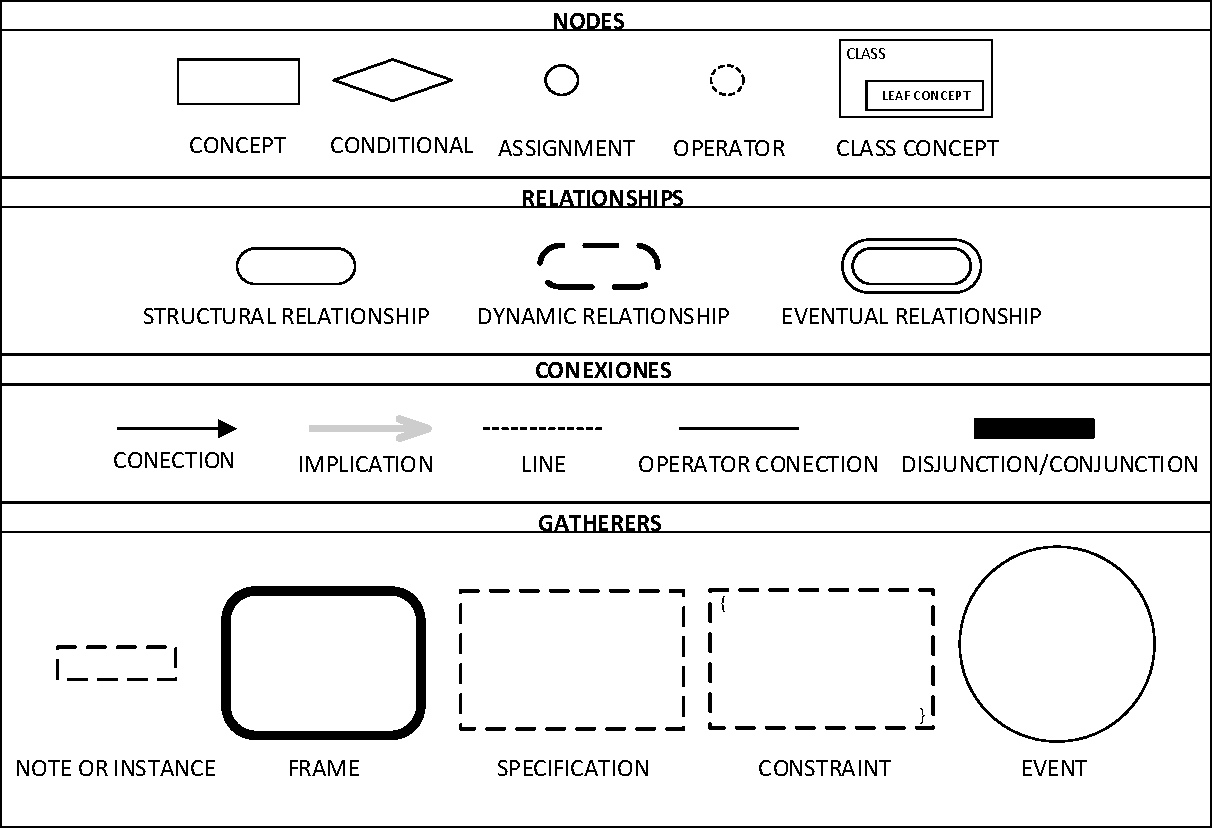
\includegraphics[width=0.7\textwidth]{Figures/PSElements.pdf}
	\caption{PS Elements by category \cite{zapata2012unc}.}
	\label{fig:PS_Elements}
\end{figure}

In addition, Calle, Chaverra and Nore\~na \cite{JCalle,norena2018Ling, JChaverra} extend the notation showed above, with elements which allow for representing domains in scientific software contexts. These elements account for usage of mathematical functions, and they allow for extending PS notation, by using user defined functions. In Figure \ref{fig:PS_Extended} we present the extended notation for PS in scientific software contexts.

\begin{figure}
	\centering
	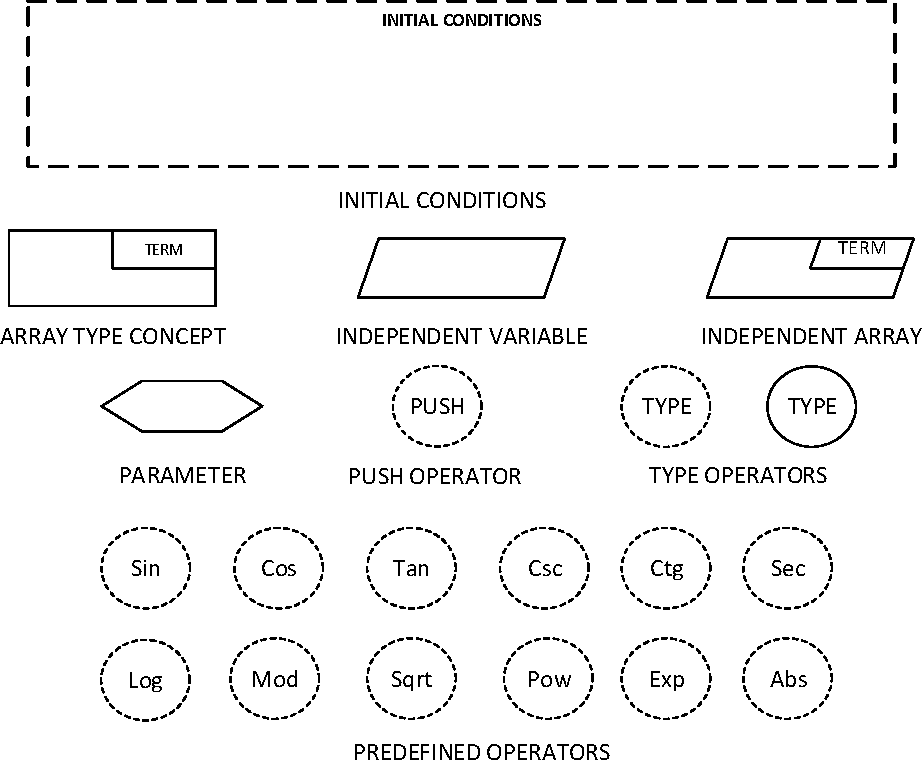
\includegraphics[width=0.7\textwidth]{Figures/PSNewElements.pdf}
	\caption{PS Extension for scientific software contexts \cite{zapata2013Eventos}}
	\label{fig:PS_Extended}
\end{figure}



\section{Event based preconceptual schema}\label{sec:representation}
For our PS representation, we first collect common concepts and synonyms across several references such as \cite{jamal2006petroleum,Bear2018,ertekin2001basic,Cao2002,Flemisch2011,HerreraCG2016,IsazaCN2017,Mohammad2017,MozoID2017,Qiao2017,cao2002development}, then search the ownership and hierarchy relationships among those concepts. These led to structural relationships in PS representation. After establishing those, we define the possible interactions between actors and concepts involved in our simulation, which are the dynamical relationships in the PS, these represent the actions in which an engineer provides the initial status of a reservoir. Once provided the initial status, some events represent the spontaneous process in which the oil reservoir changes its status, those are triggered by the pass of time, which is an event itself.\\ 
 
Our PS representation consists of seven main concepts: Mesh, Phase, Equilibrium Relationship, Interphase Interaction, Well, Rock and Equation. Moreover, three events describe the process for solving an implicit Black Oil simulation: Mesh appears, Time passes, and Phase pressure varies. 

\subsection{Mesh}
The reservoir, which is our spatial domain, is discretized as an orthogonal mesh. This mesh is a collection of cells, which are, likewise, a collection of faces forming a closed surface. In addition, when discretizing the spatial domain, properties like volume and area arise. The volumes are saved for each cell, and the areas are saved for each face. 

Moreover each cell has a numeration, which indicates its position in space, and it is used for locating the corresponding neighborhood. This is a reference to another cell, and it is saved inside the connecting face. 

For generating the simulation mesh, a geomodeller provides the quantity of cells in each direction (x,y,z), dimensions of each cell, and a top, which is the depth of the superior face of each cell. With this information, the mesh appears in an iterative process of creating cells and faces holding the cells connectivity.

\subsection{Phase}

\newpage
\newgeometry{top=0.5mm, bottom=2.5cm, left=0.5mm, right=0.5mm}
\begin{figure}
	\centering
	\includegraphics[width=1.0\textwidth]{Figures/Translated_PS.pdf}
	\caption{Black Oil PS Representation.}
	\label{fig:PS_Translated}
\end{figure}
\newpage
\restoregeometry
\section{Results}\label{sec:validation}
We developed a simulator, which code is a translation of our PS representation; We chose C++17 because of the Standard Template Library (STL) data structures, which allow for achieving a explicit consistency between the code and our PS. Moreover, the concepts are stored in global arrays, and their relations are translated as pointers. This code is available in a GitHub repository.

Here, We present some code snippets like concepts, functions or PS pieces with their representation in PS for verifying consistency. 



\begin{figure}
	\centering
	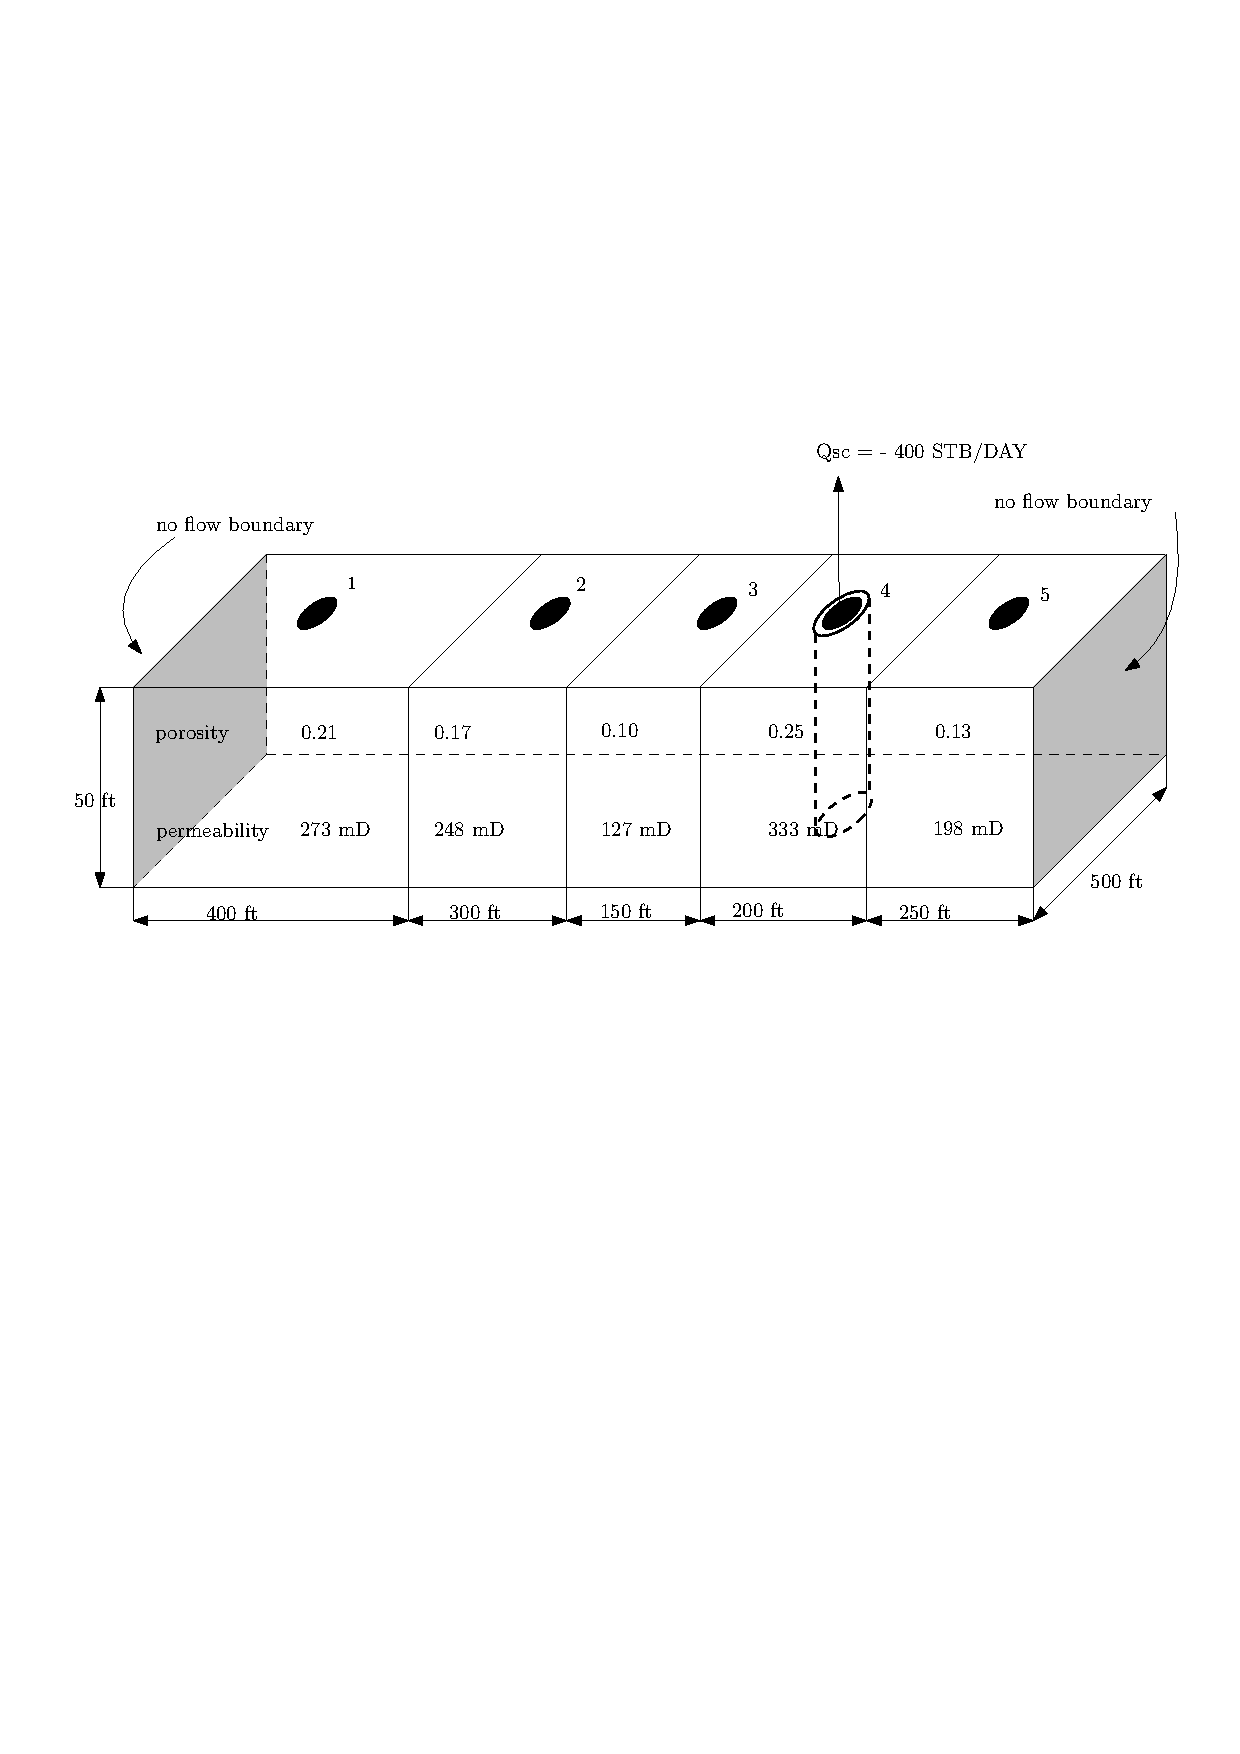
\includegraphics[width=1.0\textwidth]{Figures/casoasis.pdf}
	\caption{Graphical explanation of study case used from \cite{jamal2006petroleum}.}
	\label{fig:casoasis}
\end{figure}

\begin{figure}
	\centering
	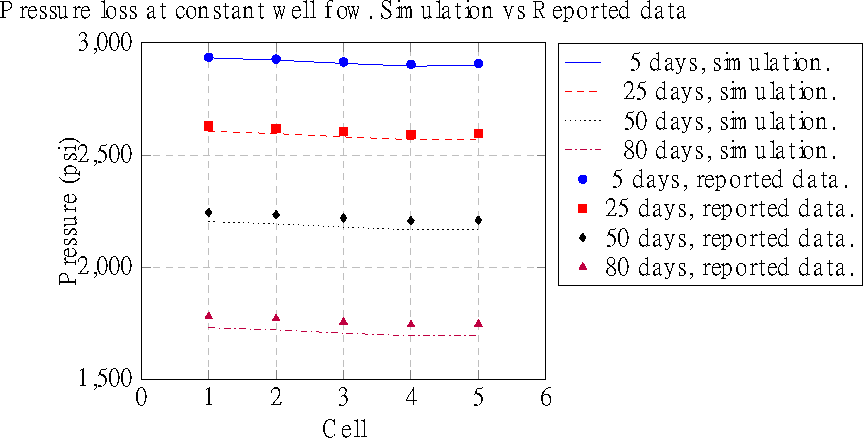
\includegraphics[width=1.0\textwidth]{Figures/Validation1.pdf}
	\caption{Pressure loss at constant well flow, simulation vs study case \cite{jamal2006petroleum}.}
	\label{fig:validation1}
\end{figure}

\begin{figure}
	\centering
	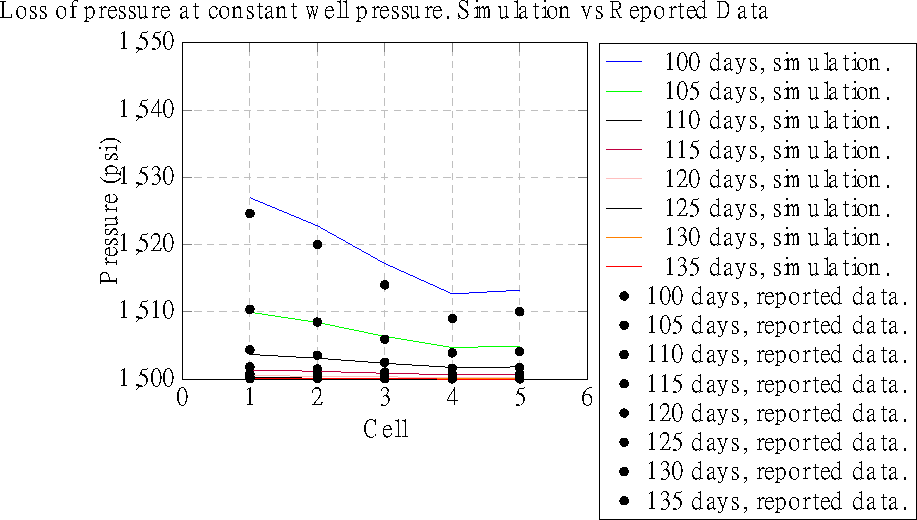
\includegraphics[width=1.0\textwidth]{Figures/Validation2.pdf}
	\caption{Pressure loss at constant well pressure, simulation vs study case \cite{jamal2006petroleum}.}
	\label{fig:validation2}
\end{figure}


\section{Conclusion}\label{sec:conclusions}

\section*{Acknowledgments}
Authors thank to FONDO NACIONAL DE FINANCIAMIENTO PARA LA CIENCIA, LA TECNOLOG\'{I}A Y LA INOVACI\'{O}N \say{FRANCISCO JOS\'{E} DE CALDAS}, to MINCIENCIAS and the Agencia Nacional de Hidrocarburos (ANH) for financial support under Contract No. 273-2017: \textit{Plan Nacional para el Potenciamiento de la Tecnolog\'{i}a CEOR con Gas Mejorado Qu\'{i}micamente}. Authors also thank Universidad Nacional de Colombia for logistic and financial support, and the research groups Flow and Transport Dynamics in porous media, and Computational Languages for their contributions on this work.

\bibliography{BibliMSc}

\end{document}